\documentclass{beamer}

\usepackage[utf8]{inputenc}
\usepackage{default}
\usepackage[T1]{fontenc}%
\usepackage{amssymb}
\usepackage{array}
\usepackage{amsmath}
\usepackage{graphicx}
\usepackage[french]{babel}
\usetheme{Berlin}
\useoutertheme{split}
\definecolor{grenat}{RGB}{139,26,26}
\definecolor{beige}{RGB}{255,255,220}

\title{\textbf{Détection du tempo et du rythme dans un morceau de musique}}
\author{Joshua Peignier \and Estelle Varloot}

\setbeamercolor{structure}{fg = grenat}
\setbeamercolor{background canvas}{bg = beige}

\defbeamertemplate*{footline}{shadow theme}
{%
  \leavevmode%
  \hbox{\begin{beamercolorbox}[wd=.5\paperwidth,ht=2.5ex,dp=1.125ex,leftskip=.3cm plus1fil,rightskip=.3cm]{author in head/foot}%
    \usebeamerfont{author in head/foot}\insertframenumber\,/\,\inserttotalframenumber\hfill\insertshortauthor
  \end{beamercolorbox}%
  \begin{beamercolorbox}[wd=.5\paperwidth,ht=2.5ex,dp=1.125ex,leftskip=.3cm,rightskip=.3cm plus1fil]{title in head/foot}%
    \usebeamerfont{title in head/foot}\insertshorttitle%
  \end{beamercolorbox}}%
  \vskip0pt%
}

\begin{document}
\frame{\titlepage}

\begin{frame}
       \tableofcontents
\end{frame}


\section{Introduction}
\begin{frame}
       \tableofcontents[currentsection]
\end{frame}


\begin{frame}
 \frametitle{Qu'est-ce que le rythme ?}
 \begin{itemize}
  \item<2-> Notion empirique \onslide<3->{$\rightarrow$ Difficilement formalisable}
  \item<4-> Globalement : la fréquence auquel on tape du pied pour accompagner un morceau
  \item<5-> Pour les musiciens : à rapprocher de la pulsation
  \item<6-> Comment extraire le rythme d'un morceau ?
 \end{itemize}
\end{frame}

\begin{frame}
 \frametitle{Problème difficile}
 \begin{itemize}
  \item Intuitivement : le rythme est un objet périodique.
  \item<2-> On peut s'attendre à trouver des pics aux fréquences concernées dans le spectre du signal
  \item<3-> Trop peu d'information exploitable en pratique
  \item<4-> Nécessité de transformer le signal reçu
 \end{itemize}
\end{frame}

\setbeamercolor{background canvas}{bg = white}
\begin{frame}
\begin{center}
 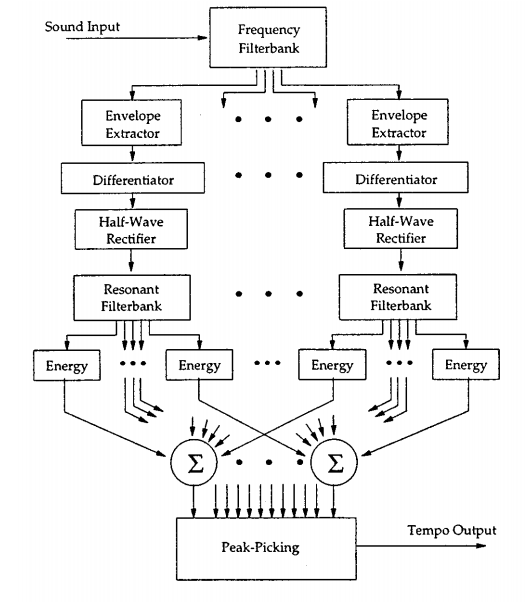
\includegraphics[scale = 0.3]{Algo.png}
\end{center}
 \end{frame}
 
 \setbeamercolor{background canvas}{bg = beige}


 \section{Idées de l'algorithme}
 \begin{frame}
       \tableofcontents[currentsection]
\end{frame}


 \begin{frame}
  \begin{itemize}
  \item Information intéressante : \onslide<2->{Intuitivement, l'enveloppe du signal}
  \item<3-> Selon le morceau : plusieurs enveloppes possibles
  \item<4-> Nécessité de séparer le spectre en bandes de fréquences
  \item<5-> Utilisation d'un banc de filtres
  \item<6-> Extraction d'enveloppe par bandes
  \end{itemize}
 \end{frame}

 \begin{frame}
  \begin{itemize}
   \item Le rythme : deux informations
   \begin{itemize}
   \item<2-> La fréquence de la pulsation
   \item<3-> La phase de la pulsation
   \end{itemize}
   \item<4-> Pour la détection : nécessiter de trouver la phase
  \end{itemize}

 \end{frame}

\end{document}
